El \pArm{} se basa en el trabajo inicial del $\mu$Arm, no utilizando directamente lo desarrollado por la empresa UFACTORY sino aprovechando el trabajo ya realizado y los recursos disponibles para estudiarlos. Si bien es cierto que el $\mu$Arm ya es un sistema avanzado y capaz, como se explicó en la Introducción (\ref{ch:intro}), se pretende estudiar y desarrollar un sistema propio el cual pueda servir para ayudar y facilitar la entrada a este tipo de tecnologías a otras personas, haciéndolo comprensible y, aprovechando la tecnología de la impresión en 3D, fabricable por uno mismo.

Además, en relación a los \ac{ODS}, con el desarrollo de este sistema se pretende trabajar en:

\begin{itemize}
    \item [4 -] Educación de Calidad\footnote{\url{https://www.un.org/sustainabledevelopment/es/education/}}.
    \item [7 -] Energía Asequible y No Contaminante\footnote{\url{https://www.un.org/sustainabledevelopment/es/energy/}}.
    \item [10 -] Reducción de las desigualdades\footnote{\url{https://www.un.org/sustainabledevelopment/es/inequality/}}.
\end{itemize}

Para el primero, se tiene en cuenta que el producto se desarrollará siguiendo las iniciativas \ac{OS} y \ac{OH}, las cuales facilitan el acceso a la información a cualquiera que la requiera. Además, se facilitará el desarrollo al completo detallado y explicado, con la resolución de los problemas pertinentes y el porqué de ella.

Para el segundo, el \pArm{} utilizará la electricidad como fuente de energía, evitando así otras más contaminantes como las producidas por combustibles fósiles. En añadido, se trabajará para que el consumo de energía sea el menor posible, permitiendo así un mayor tiempo de uso con la misma fuente de alimentación y no abusando de los recursos de los que se disponen.

Finalmente, se pretende hacer que el \pArm{} tenga un coste bajo, permitiendo así el acceso a los recursos y los procesos de fabricación a todo el mundo que pudiera estar interesado y que disponga de la cantidad mínima necesaria para poder poner en funcionamiento el brazo robótico.

Por otra parte, el \pArm{} es dependiente de otro sistema que lo controle, ya que no se plantea como sistema autónomo. Por consiguiente, se proponen diversos métodos de conexión entre el brazo y dicho sistema. Por ejemplo, se puede utilizar el puerto serie \ac{USB} o bien comunicaciones inalámbricas, como \textit{Bluetooth} y \textit{WiFi}. Además, debido a su disponibilidad multiplataforma, se propone el uso de Python como alternativa de programación.

De ahora en adelante, se denominará ``\ac{S1}'' al equipo que controla al \pArm{}; y ``\ac{S2}'' al brazo robótico en sí.

Para este proyecto, se ha de desarrollar el \ac{SW} que se ejecutará en \ac{S1}, además de tanto el \ac{SW} como el \ac{HW} que irán en \ac{S2}, adaptando la estructura mecánica para funcionar con una impresora.

\subsection{Interfaz del sistema}
En un principio, el sistema estará dividido en dos módulos:

\subsection*{\ac{S1}}
\ac{S1} consiste en un equipo el cual controlará el brazo robótico (\ac{S2}). Para ello, tal y como se planteó anteriormente, se propone como lenguaje de programación Python, el cual soporta la ejecución con \ac{GUI}.

En lo referente al sistema operativo, al ser una aplicación en Python la cual es multiplataforma, no se define ninguna restricción respecto al mismo.

Finalmente, se plantea la conexión con \ac{S2} utilizando el puerto serie \ac{USB}, por lo que también será necesario que el equipo anfitrión \ac{S1} disponga de una conexión de ese estilo.

En resumen (ver la tabla \ref{tab:s1_requirements}):

\begin{table}[H]
    \centering
    \begin{tabularx}{\textwidth}{| c | X | X |}
        \hline
        \textbf{Componente} & \textbf{Función} & \textbf{Restricciones} \\
        \hline\hline
        Sistema Operativo & Hospedar y ejecutar la aplicación Python que controlará el brazo robótico. & Debe poder ejecutar aplicaciones Python con \ac{GUI}, por ejemplo, \ac{GTK}. \\
        \hline
        \textit{Conexión con \ac{S2}} & Permitir la comunicación con el sistema \ac{S2} en modo dúplex. & Velocidad adaptable (\textit{baud--rate)} y capacidad para gran ancho de banda. \\
        \hline
        Python & Control del sistema \ac{S2} y monitorización del estado del mismo. & Versión Python $\geqslant$ 3.6.* \\
        \hline
    \end{tabularx}
    \caption{Requisitos del sistema \ac{S1}.}
    \label{tab:s1_requirements}
\end{table}

En principio, no será necesaria la conexión a Internet, pero tampoco se descarta el uso de la misma a la hora de poder recibir actualizaciones o en lo referente a futuras mejoras.

\subsection*{\ac{S2}}
Para el sistema \ac{S2} no se ha pensado en ningún microprocesador ni \ac{SoC} en particular, pero se han contemplado algunos que cumplen con las características requeridas (ver la tabla \ref{tab:s2_chips}).

Será necesario que el circuito escogido disponga de algún tipo de entrada de las propuestas para la comunicación con \ac{S1}. Debido a la característica descrita en la tabla \ref{tab:s1_requirements} sobre la interfaz de comunicación, no será estrictamente necesario que la velocidad sea adaptable (ya que se asume que se adaptará en \ac{S1}); sin embargo, sí será requisito fundamental que la conexión sea dúplex y que soporte gran cantidad de datos con las menores pérdidas posibles.

Por otra parte, el microcontrolador deberá poder modular señales \ac{PWM} para controlar los distintos motores de los que dispondrá el brazo. Sin embargo, en caso de que finalmente el \textit{chip} escogido no disponga de dicha modularización, se podrán usar motores que cuenten con un \textit{driver} que permitan controlarlos usando señales digitales y/o analógicas.

Teniendo en cuenta lo anterior, se plantea el uso de los siguientes dispositivos (ver tabla \ref{tab:s2_chips}):

\begin{table}[H]
    \centering
    \begin{tabularx}{\textwidth}{| c | X | X | X |}
        \hline
        \textbf{Placa} & \textbf{Ventajas} & \textbf{Desventajas} & \textbf{ID \textit{RS--Online} y precio} \\
        \hline
        ESP8266 & \ac{SoC} bastante barato (5\EUR{}) con conexión WiFi y modo de bajo consumo & Señal \ac{PWM} generada por \ac{SW}; poca cantidad de \ac{GPIO} (6). & 124-5505 -- 19,29\EUR{} \\
        \hline
        ESP32 & \ac{SoC} con procesador de dos núcleos que permite comunicaciones WiFi y Bluetooth & No cuenta con \ac{GPIO} pero permite la comunicación mediante el protocolo I²C. & 188-5441 -- 25,29\EUR{} \\
        \hline
        PIC16F18326-I/P & Microcontrolador de 8 bits de baja potencia de consumo y bajo precio con capacidad de modularizar hasta dos señales \ac{PWM} y con más memoria RAM que otros componentes de su familia. Finalmente, cuenta con bastantes salidas \ac{GPIO}, suficientes como para añadir más componentes al sistema. & No está integrada en una placa (\ac{SoC}) por lo que habría que hacer toda la lógica del diseño \ac{HW}. No dispone de conexiones de red (aunque no son necesarias) y la capacidad de cómputo, en comparación con las otras propuestas, es menor. & 124-1554 -- 1,375\EUR{} \\
        \hline
        dsPIC33EP***GM604 & Microcontrolador de 16 bits con gran capacidad de cómputo matricial que, además, cuenta con un procesador digital de señales, permitiendo realizar operaciones matriciales más rápidamente. Además, cuenta con hasta 6 señales \ac{PWM} y múltiples GPIO. & Al igual que el componente anterior, no está integrado en una placa \ac{SoC} por lo que habría que diseñar toda la PCB que contenga el sistema. & 825-1023 -- 5,89\EUR{} \\
        \hline
    \end{tabularx}
    \caption{Posibles \textit{chips} que se han planteado para el proyecto.}
    \label{tab:s2_chips}
\end{table}


\subsection{Interfaz de usuario}

El usuario final del producto solamente interactuara de manera directa con \ac{S1}.
Para que esta interacción sea posible, se desarrollara un panel de control que permita al usuario definir movimientos que el robot deberá realizar. El panel de control se mostrará en una sola pantalla y permitirá al usuario, mediante una interfaz gráfica sencilla, mover de manera independiente cada uno de los motores del robot, o bien mediante el uso del ratón, describir trayectorias que el robot realizara en tiempo real replicando el movimiento del ratón.

Además, también se podrá desplazar el robot indicando la posición $\left\{x, y, z\right\}$ referente al \textit{end--effector}. Se sugiere una interfaz que siga el siguiente diseño:

\begin{figure}[H]
    \centering
    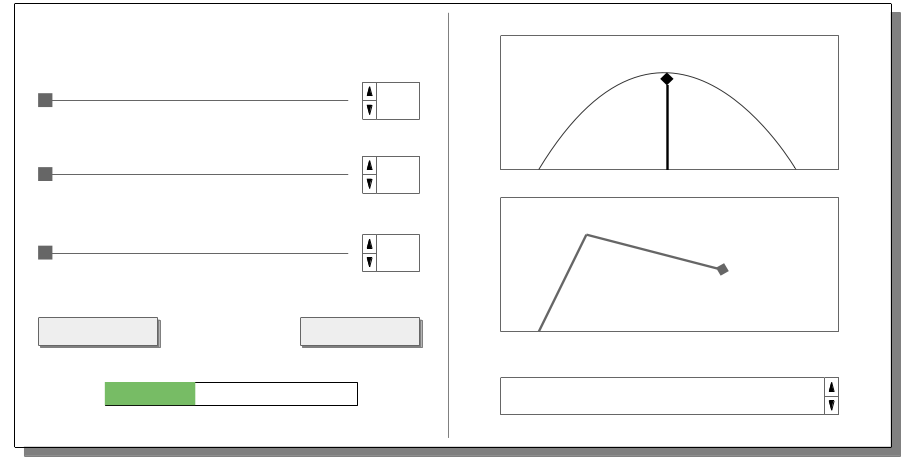
\includegraphics[width=\linewidth]{RS/images/InterfaceSketch-MkII.png}
    \caption{Diseño propuesto para la intefaz gráfica de usuario.}
    \label{fig:ui_design}
\end{figure}

La especificación de los elementos de la interfaz anterior (figura \ref{fig:ui_design}) se hace en mayor profundidad en el punto \ref{sec:ui_reqs} del documento.

\subsection{Memoria}

Dado que se pretende que todo el código de control y de cálculo matricial vaya dentro de \ac{S2}, se tienen las restricciones de memoria del mismo. En este caso, se estaría limitado a la capacidad de los
distintos microcontroladores que se especificaron en la tabla \ref{tab:s2_chips}.

Como, por lo general, se suele trabajar con microcontroladores de Microchip en
la Universidad, se van a asumir las restricciones de memoria del dsPIC33EP512GM604,
las cuales consisten en:

\begin{itemize}
    \item 512 KB de memoria \textit{flash}, donde se alberga el programa principal.
    \item 16 KB de memoria \ac{RAM}, donde se alojarán los datos temporales durante la ejecución, en particular, las matrices de las ecuaciones cinemáticas.
\end{itemize} 

\subsection{Operaciones}

Los usuarios deberán desempeñar acciones tales que generen los movimientos deseados en el brazo. Estas acciones pueden implicar interactuar con los \textit{widgets} presentes en el panel de control o bien efectuar movimientos con el ratón para que el robot los desempeñe directamente.
